% Structure of the General Context Memory (GCM): guide table, one agent per ring,
% regions with concentric rings. Redrawn after Fig. 2 of the article.
\documentclass[border=0pt]{standalone}
% Shared preamble of the GSO-RL documentation figures.
% Compiled with latex (DVI) + dvisvgm; see ../build.sh.
\def\pgfsysdriver{pgfsys-dvisvgm.def}
\usepackage[T1]{fontenc}
\usepackage{lmodern}
\renewcommand{\familydefault}{\sfdefault}
\usepackage{amsmath, amssymb}
\usepackage{tikz}
\usetikzlibrary{positioning, shapes, arrows.meta, calc, fit, backgrounds}

% Palette
\definecolor{Purple}{RGB}{102, 0, 153}
\colorlet{ColMa}{green!50!black}   % macro-move M1
\colorlet{ColMb}{blue!70!black}    % macro-move M2
\colorlet{ColMc}{orange!85!black}  % macro-move M3
\definecolor{cGa}{RGB}{38, 166, 154}
\definecolor{cGb}{RGB}{229, 96, 76}
\definecolor{cGc}{RGB}{235, 165, 40}
\definecolor{cGd}{RGB}{125, 125, 215}
\definecolor{cGe}{RGB}{190, 60, 150}

% White background so figures stay readable in dark mode. The white rectangle lives on the
% "background" layer; figures draw their own backdrops on "behind", which sits above it.
\pgfdeclarelayer{behind}
\pgfsetlayers{background,behind,main}
\tikzset{every picture/.append style={show background rectangle,
  background rectangle/.style={fill=white, draw=none}, inner frame sep=8pt}}
% NOTE: with dvisvgm, text placed after a \color{...} group inside the same node is misplaced.
% Put differently coloured pieces of text in separate nodes.

\newcommand{\yes}{{\color{green!50!black}\checkmark}}
\newcommand{\nope}{{\color{red!70!black}$\boldsymbol{\times}$}}

% A region: guide with three concentric rings.  \guia[style]{x}{y}{color}{label}
\newcommand{\guia}[5][]{%
  \fill[#4!10, #1] (#2,#3) circle (1.05);
  \fill[#4!20, #1] (#2,#3) circle (0.7);
  \fill[#4!35, #1] (#2,#3) circle (0.35);
  \foreach \r in {0.35,0.7,1.05} \draw[#4, #1] (#2,#3) circle (\r);
  \fill[#4!80!black, #1] (#2,#3) circle (2pt);
  \node[#4!75!black, font=\scriptsize\bfseries, #1] at (#2,#3+1.22) {#5};
}

\begin{document}
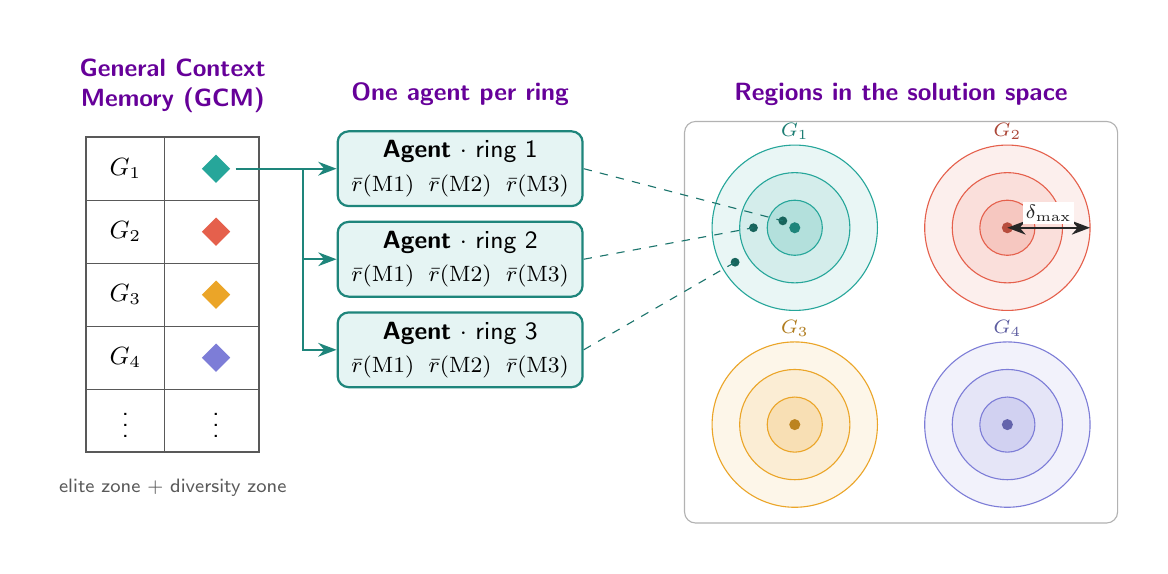
\begin{tikzpicture}[>=Stealth, font=\small,
  agent/.style={rectangle, rounded corners, draw=cGa!80!black, fill=cGa!12, thick,
                text width=2.9cm, align=center, minimum height=0.95cm, inner sep=3pt}]
  % ---- Guide table ----
  \node[font=\small\bfseries, Purple, align=center] at (1.1,5.55) {General Context\\ Memory (GCM)};
  \foreach \y/\g/\c in {4.5/1/cGa, 3.7/2/cGb, 2.9/3/cGc, 2.1/4/cGd} {
    \node at (0.5,\y) {$G_{\g}$};
    \node[diamond, fill=\c, inner sep=2.6pt] at (1.65,\y) {};
  }
  \node at (0.5,1.35) {$\vdots$};
  \node at (1.65,1.35) {$\vdots$};
  \draw[gray!70!black, thick] (0,0.9) rectangle (2.2,4.9);
  \draw[gray!70!black] (1.0,0.9) -- (1.0,4.9);
  \foreach \y in {4.1,3.3,2.5,1.7} \draw[gray!70!black] (0,\y) -- (2.2,\y);
  \node[font=\scriptsize, gray!70!black, align=center] at (1.1,0.45) {elite zone + diversity zone};

  % ---- Agents of G1 (one per ring) ----
  \node[font=\small\bfseries, Purple] at (4.75,5.45) {One agent per ring};
  \foreach \k/\y in {1/4.5, 2/3.35, 3/2.2} {
    \node[agent] (a\k) at (4.75,\y)
      {\textbf{Agent} $\cdot$ ring \k\\[1pt]
       \footnotesize $\bar r(\mathrm{M1})\;\;\bar r(\mathrm{M2})\;\;\bar r(\mathrm{M3})$};
  }
  \coordinate (hub) at (2.75,4.5);
  \draw[thick, cGa!80!black] (1.9,4.5) -- (hub);
  \foreach \k in {1,2,3} \draw[->, thick, cGa!80!black] (hub) |- (a\k.west);

  % ---- Regions in the solution space ----
  \node[font=\small\bfseries, Purple] at (10.35,5.45) {Regions in the solution space};
  \draw[gray!60, rounded corners] (7.6,0.0) rectangle (13.1,5.1);
  \guia{9.0}{3.75}{cGa}{$G_1$}
  \guia{11.7}{3.75}{cGb}{$G_2$}
  \guia{9.0}{1.25}{cGc}{$G_3$}
  \guia{11.7}{1.25}{cGd}{$G_4$}
  \draw[<->, gray!30!black, thick] (11.7,3.75) -- (12.75,3.75)
    node[midway, above=1pt, font=\scriptsize, fill=white, inner sep=1pt] {$\delta_{\max}$};
  % links agent k -> ring k of G1
  \foreach \k/\r/\a in {1/0.175/150, 2/0.525/180, 3/0.875/210} {
    \coordinate (p\k) at ($(9.0,3.75)+(\a:\r)$);
    \fill[cGa!60!black] (p\k) circle (1.6pt);
    \draw[cGa!70!black, dashed] (a\k.east) -- (p\k);
  }
\end{tikzpicture}
\end{document}
